	\section{Identification}

\begin{center}
\scalebox{0.7}{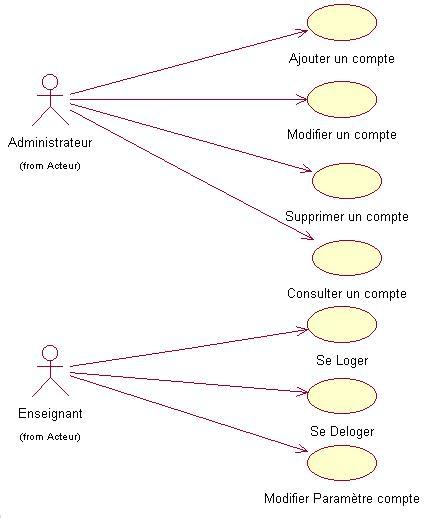
\includegraphics{images/identification.jpg}}\\
\par{Paquetage Gestion des Comptes}
\end{center}
Voici les diff{\'e}rents sc{\'e}narios:\\
	\begin{itemize}
	\item Enseignant
		\begin{itemize}
		\item Se loger :
			\begin{itemize}
			\item Pr{\'e}-requis : Avoir un compte et un mot de passe
			\item Description : L'utilisateur remplit les
			champs Login et Mot de passe dans la page d'accueil.\\
			Il valide.
			\item Post-requis : L'utilisateur est identifi{\'e} dans l'intranet.
			\end{itemize}
		\item Se d{\'e}loger :
			\begin{itemize}
			\item Pr{\'e}-requis : Etre identifi{\'e}/log{\'e}. 
			\item Description : L'utilisateur clique sur
			{\it Se d{\'e}connecter} dans la page des liens.
			\item Post-requis : L'utilisateur se trouve dans la page d'accueil de l'intranet.
			\end{itemize}
		\item Consulter son compte :
			\begin{itemize}
			\item  Pr{\'e}-requis : Etre identifi{\'e}.
			\item Description : L'utilisateur clique sur
			{\it Consulter mon compte} dans la page des liens. 
			\item Post-requis : Affichage de la page de
			consultation du compte de l'utilisateur connect{\'e}.
			\end{itemize}
		\item Modifier les param{\`e}tres :
			\begin{itemize}
			\item Pr{\'e}-requis : Etre identifi{\'e}/log{\'e}. 
			\item Description : L'utilisateur clique sur
			{\it Modifier} lors de la consultation de son compte.\\
			Dans le cas du mot de passe : il entre son
			nouveau mot de passe et le confirme.
			\item Post-requis : Les param{\`e}tres sont modifi{\'e}s.
			\end{itemize}
		\end{itemize}
	\item Administrateur
		\begin{itemize}
		\item Ajouter compte :
			\begin{itemize}
			\item Pr{\'e}-requis : Etre identifi{\'e}/log{\'e}. 
			\item Description : L'administrateur clique sur le lien {\it Ajout de compte}.\\
			Il entre dans une nouvelle page o{\`u} il doit
			remplir des champs pour le nouveau compte.\\
			Il entre un login et ajoute un mot de passe qu'il confirme.\\
			Il a la possibilit{\'e} de g{\'e}n{\'e}rer un login et
			mot de passe automatiquement (le login est g{\'e}n{\'e}r{\'e} {\`a} partir du
			nom et pr{\'e}nom de l'utilisateur. Le mot de passe est g{\'e}n{\'e}r{\'e}
			al{\'e}atoirement).\\
			Il entre {\'e}ventuellement les param{\`e}tres
			personnelles de l'utilisateur.
			\item Post-requis : Nouveau compte ajout{\'e} dans
			la base de donn{\'e}es.
			\item {\bf Remarque :} L'enseignant poss{\'e}dant
			le compte ainsi cr{\'e}{\'e} n'est rattach{\'e} {\`a} aucun
			enseignement, il peut ainsi juste
			cr{\'e}er/modifier/supprimer des exercices (s'il
			est propri{\'e}taire pour la suppression et la modfication).  
			\end{itemize}

		\item Rechercher compte :
			\begin{itemize}
			\item Pr{\'e}-requis : Etre identifi{\'e}/log{\'e}. 
			\item Description : L'administrateur clique
			sur le lien {\it Rechercher compte}. Il a la
			possibilit{\'e} de rechercher soit par nom soit
			par login ou peut tout simplement lister tous
			les comptes existants (affichage par ordre
			alphab{\'e}tique des noms ou login, au choix).
			\item Post-requis : Un listing du ou des
			comptes recherch{\'e}s s'affiche(nt) s'il(s)
			existe(nt) dans la base.
			\end{itemize}

		\item Modifier compte :
			\begin{itemize}
			\item Pr{\'e}-requis : Etre log{\'e}/identifi{\'e}. 
			\item Description : L'administrateur recherche
			le compte voulu puis clique sur le lien {\it
			Modifier} ({\`a} c{\^o}t{\'e} du lien vers le compte).\\
			(Il a la possibilit{\'e} de modifier le compte lors
			de la consultation.)
			Il entre dans la page de modification de compte.\\
			Il a la possibilit{\'e} de modifier les param{\`e}tres
			du compte.\\
			L'administrateur a la possibilit{\'e}
			d'ajouter/retirer des droits sur des
			enseignements (voir dans {\bf Gestion des droits}).
			\item Post-requis : Le compte est modifi{\'e} dans la base. 
			\end{itemize}

		\item Consulter un compte quelconque:
			\begin{itemize}
			\item Pr{\'e}-requis : Etre log{\'e}/identifi{\'e}. 
			\item Description : L'administrateur recherche
			le compte voulu puis clique sur le lien {\it
			Consulter} {\`a} c{\^o}t{\'e} du compte.\\
			Il entre dans la page de consultation du compte.
			\item Post-requis : Il obtient la page de consultation.\\
			La base de donn{\'e}e reste inchang{\'e}.
			\end{itemize}

		\item {\bf Supprimer compte} :
			\begin{itemize}
			\item {\bf Pr{\'e}-requis} : Etre log{\'e}/identifi{\'e}.
			\item {\bf Description} : L'administrateur recherche
			le compte voulu puis clique sur le lien {\it
			Supprimer} {\`a} c{\^o}t{\'e} du compte.\\
			Il est redirig{\'e} vers une page de
			confirmation o{\`u} il valide.\\ Il a la
			possiblit{\'e} de supprimer le compte lors de la consultation.
			\item {\bf Post-requis} : Suppression du compte
			selectionn{\'e} dans la base de donn{\'e}e\\
			\end{itemize}
		\end{itemize}
	\end{itemize}
\newpage
Voyons maintenant les priorit{\'e}s des diff{\'e}rentes actions quant au
d{\'e}veloppement du logiciel.\\\\\\
\begin{tabular}{|p{4cm}|c|p{4cm}|p{5cm}|}
\hline
  Fonction & Priorit{\'e} & Qualit{\'e} & Mesure \\
\hline
Ajouter un compte &  5 & Fiabilit{\'e} & Coh{\'e}rence entre les logins et les mots de passe. \\
\hline
Modifier un compte & 3 & Fiabilit{\'e} & Coh{\'e}rence entre les logins et les
  mots de passe. \\
\hline
Rechercher un compte & 5 & Fiabilit{\'e} & Coh{\'e}rence entre la requ{\^e}te demand{\'e}e et la r{\'e}ponse donn{\'e}e. \\
\hline
Consulter un compte quelconque & 2 & Sur. S{\'e}curit{\'e} & Eviter toutes erreurs de l'administrateur. \\
\hline
Consulter son compte & 3 & S{\'e}curit{\'e} & \\
\hline
Supprimer un compte & 4 & S{\'e}curit{\'e}. Fiabilit{\'e} & Ne pas supprimer
  d'autres comptes que celui s{\'e}lectionn{\'e}.\\
\hline
Se loger & 5 & S{\'e}curit{\'e}. Fiabilit{\'e} & Se connecter au compte entr{\'e}.\\
\hline
Se d{\'e}loger  & 5 & S{\'e}curit{\'e}. Fiabilit{\'e} &  D{\'e}connexion assur{\'e}e. Ne pas pouvoir d{\'e}loger en m{\^e}me temps d'autres personnes connect{\'e}es sur l'application.\\
\hline
Modifier param{\`e}tres compte  & 3 & s{\'e}curit{\'e},fiabilit{\'e} & Garantir une 
  s{\'e}curit{\'e}. Le nouveau mot de passe ne peut pas {\^e}tre intercept{\'e}. Garantir la validit{\'e} du mot de passe  \\
\hline
\end{tabular}










